% Options for packages loaded elsewhere
\PassOptionsToPackage{unicode}{hyperref}
\PassOptionsToPackage{hyphens}{url}
\PassOptionsToPackage{dvipsnames,svgnames,x11names}{xcolor}
%
\documentclass[
  letterpaper,
  DIV=11,
  numbers=noendperiod]{scrreport}

\usepackage{amsmath,amssymb}
\usepackage{iftex}
\ifPDFTeX
  \usepackage[T1]{fontenc}
  \usepackage[utf8]{inputenc}
  \usepackage{textcomp} % provide euro and other symbols
\else % if luatex or xetex
  \usepackage{unicode-math}
  \defaultfontfeatures{Scale=MatchLowercase}
  \defaultfontfeatures[\rmfamily]{Ligatures=TeX,Scale=1}
\fi
\usepackage{lmodern}
\ifPDFTeX\else  
    % xetex/luatex font selection
\fi
% Use upquote if available, for straight quotes in verbatim environments
\IfFileExists{upquote.sty}{\usepackage{upquote}}{}
\IfFileExists{microtype.sty}{% use microtype if available
  \usepackage[]{microtype}
  \UseMicrotypeSet[protrusion]{basicmath} % disable protrusion for tt fonts
}{}
\makeatletter
\@ifundefined{KOMAClassName}{% if non-KOMA class
  \IfFileExists{parskip.sty}{%
    \usepackage{parskip}
  }{% else
    \setlength{\parindent}{0pt}
    \setlength{\parskip}{6pt plus 2pt minus 1pt}}
}{% if KOMA class
  \KOMAoptions{parskip=half}}
\makeatother
\usepackage{xcolor}
\setlength{\emergencystretch}{3em} % prevent overfull lines
\setcounter{secnumdepth}{-\maxdimen} % remove section numbering
% Make \paragraph and \subparagraph free-standing
\makeatletter
\ifx\paragraph\undefined\else
  \let\oldparagraph\paragraph
  \renewcommand{\paragraph}{
    \@ifstar
      \xxxParagraphStar
      \xxxParagraphNoStar
  }
  \newcommand{\xxxParagraphStar}[1]{\oldparagraph*{#1}\mbox{}}
  \newcommand{\xxxParagraphNoStar}[1]{\oldparagraph{#1}\mbox{}}
\fi
\ifx\subparagraph\undefined\else
  \let\oldsubparagraph\subparagraph
  \renewcommand{\subparagraph}{
    \@ifstar
      \xxxSubParagraphStar
      \xxxSubParagraphNoStar
  }
  \newcommand{\xxxSubParagraphStar}[1]{\oldsubparagraph*{#1}\mbox{}}
  \newcommand{\xxxSubParagraphNoStar}[1]{\oldsubparagraph{#1}\mbox{}}
\fi
\makeatother


\providecommand{\tightlist}{%
  \setlength{\itemsep}{0pt}\setlength{\parskip}{0pt}}\usepackage{longtable,booktabs,array}
\usepackage{calc} % for calculating minipage widths
% Correct order of tables after \paragraph or \subparagraph
\usepackage{etoolbox}
\makeatletter
\patchcmd\longtable{\par}{\if@noskipsec\mbox{}\fi\par}{}{}
\makeatother
% Allow footnotes in longtable head/foot
\IfFileExists{footnotehyper.sty}{\usepackage{footnotehyper}}{\usepackage{footnote}}
\makesavenoteenv{longtable}
\usepackage{graphicx}
\makeatletter
\def\maxwidth{\ifdim\Gin@nat@width>\linewidth\linewidth\else\Gin@nat@width\fi}
\def\maxheight{\ifdim\Gin@nat@height>\textheight\textheight\else\Gin@nat@height\fi}
\makeatother
% Scale images if necessary, so that they will not overflow the page
% margins by default, and it is still possible to overwrite the defaults
% using explicit options in \includegraphics[width, height, ...]{}
\setkeys{Gin}{width=\maxwidth,height=\maxheight,keepaspectratio}
% Set default figure placement to htbp
\makeatletter
\def\fps@figure{htbp}
\makeatother
% definitions for citeproc citations
\NewDocumentCommand\citeproctext{}{}
\NewDocumentCommand\citeproc{mm}{%
  \begingroup\def\citeproctext{#2}\cite{#1}\endgroup}
\makeatletter
 % allow citations to break across lines
 \let\@cite@ofmt\@firstofone
 % avoid brackets around text for \cite:
 \def\@biblabel#1{}
 \def\@cite#1#2{{#1\if@tempswa , #2\fi}}
\makeatother
\newlength{\cslhangindent}
\setlength{\cslhangindent}{1.5em}
\newlength{\csllabelwidth}
\setlength{\csllabelwidth}{3em}
\newenvironment{CSLReferences}[2] % #1 hanging-indent, #2 entry-spacing
 {\begin{list}{}{%
  \setlength{\itemindent}{0pt}
  \setlength{\leftmargin}{0pt}
  \setlength{\parsep}{0pt}
  % turn on hanging indent if param 1 is 1
  \ifodd #1
   \setlength{\leftmargin}{\cslhangindent}
   \setlength{\itemindent}{-1\cslhangindent}
  \fi
  % set entry spacing
  \setlength{\itemsep}{#2\baselineskip}}}
 {\end{list}}
\usepackage{calc}
\newcommand{\CSLBlock}[1]{\hfill\break\parbox[t]{\linewidth}{\strut\ignorespaces#1\strut}}
\newcommand{\CSLLeftMargin}[1]{\parbox[t]{\csllabelwidth}{\strut#1\strut}}
\newcommand{\CSLRightInline}[1]{\parbox[t]{\linewidth - \csllabelwidth}{\strut#1\strut}}
\newcommand{\CSLIndent}[1]{\hspace{\cslhangindent}#1}

\KOMAoption{captions}{tableheading}
\makeatletter
\@ifpackageloaded{bookmark}{}{\usepackage{bookmark}}
\makeatother
\makeatletter
\@ifpackageloaded{caption}{}{\usepackage{caption}}
\AtBeginDocument{%
\ifdefined\contentsname
  \renewcommand*\contentsname{Table des matières}
\else
  \newcommand\contentsname{Table des matières}
\fi
\ifdefined\listfigurename
  \renewcommand*\listfigurename{Liste des Figures}
\else
  \newcommand\listfigurename{Liste des Figures}
\fi
\ifdefined\listtablename
  \renewcommand*\listtablename{Liste des Tables}
\else
  \newcommand\listtablename{Liste des Tables}
\fi
\ifdefined\figurename
  \renewcommand*\figurename{Figure}
\else
  \newcommand\figurename{Figure}
\fi
\ifdefined\tablename
  \renewcommand*\tablename{Table}
\else
  \newcommand\tablename{Table}
\fi
}
\@ifpackageloaded{float}{}{\usepackage{float}}
\floatstyle{ruled}
\@ifundefined{c@chapter}{\newfloat{codelisting}{h}{lop}}{\newfloat{codelisting}{h}{lop}[chapter]}
\floatname{codelisting}{Listing}
\newcommand*\listoflistings{\listof{codelisting}{Liste des Listings}}
\makeatother
\makeatletter
\makeatother
\makeatletter
\@ifpackageloaded{caption}{}{\usepackage{caption}}
\@ifpackageloaded{subcaption}{}{\usepackage{subcaption}}
\makeatother

\ifLuaTeX
\usepackage[bidi=basic]{babel}
\else
\usepackage[bidi=default]{babel}
\fi
\babelprovide[main,import]{french}
% get rid of language-specific shorthands (see #6817):
\let\LanguageShortHands\languageshorthands
\def\languageshorthands#1{}
\ifLuaTeX
  \usepackage{selnolig}  % disable illegal ligatures
\fi
\usepackage{bookmark}

\IfFileExists{xurl.sty}{\usepackage{xurl}}{} % add URL line breaks if available
\urlstyle{same} % disable monospaced font for URLs
% Make links footnotes instead of hotlinks:
\DeclareRobustCommand{\href}[2]{#2\footnote{\url{#1}}}
\hypersetup{
  pdftitle={IR٭ Huma-Num~: Trouvez votre consortium et utilisez les outils disponibles},
  pdfauthor={Julien Rabaud},
  pdflang={fr},
  colorlinks=true,
  linkcolor={blue},
  filecolor={Maroon},
  citecolor={Blue},
  urlcolor={Blue},
  pdfcreator={LaTeX via pandoc}}


\title{IR٭ \textbf{Huma-Num}~:Trouvez votre \textbf{consortium} et
utilisez les \textbf{outils} disponibles}
\usepackage{etoolbox}
\makeatletter
\providecommand{\subtitle}[1]{% add subtitle to \maketitle
  \apptocmd{\@title}{\par {\large #1 \par}}{}{}
}
\makeatother
\subtitle{UPPA - ED 481 SSH / Outils pour les humanités numériques}
\author{Julien Rabaud}
\date{2024-11-18}

\begin{document}
\maketitle

\renewcommand*\contentsname{Table des matières}
{
\hypersetup{linkcolor=}
\setcounter{tocdepth}{2}
\tableofcontents
}
\listoffigures
\listoftables

\bookmarksetup{startatroot}

\chapter{Accueil}\label{accueil}

\begin{center}

\includegraphics{IMG/HN_LOGO_COULEUR-RVB_Logo-scaled.jpg}
\end{center}

\subsection{\texorpdfstring{Des outils et des services numériquespour
manipuler et produire des données
\textbf{FAIR}}{Des outils et des services numériques pour manipuler et produire des données FAIR}}\label{des-outils-et-des-services-numuxe9riques-pour-manipuler-et-produire-des-donnuxe9es-fair}

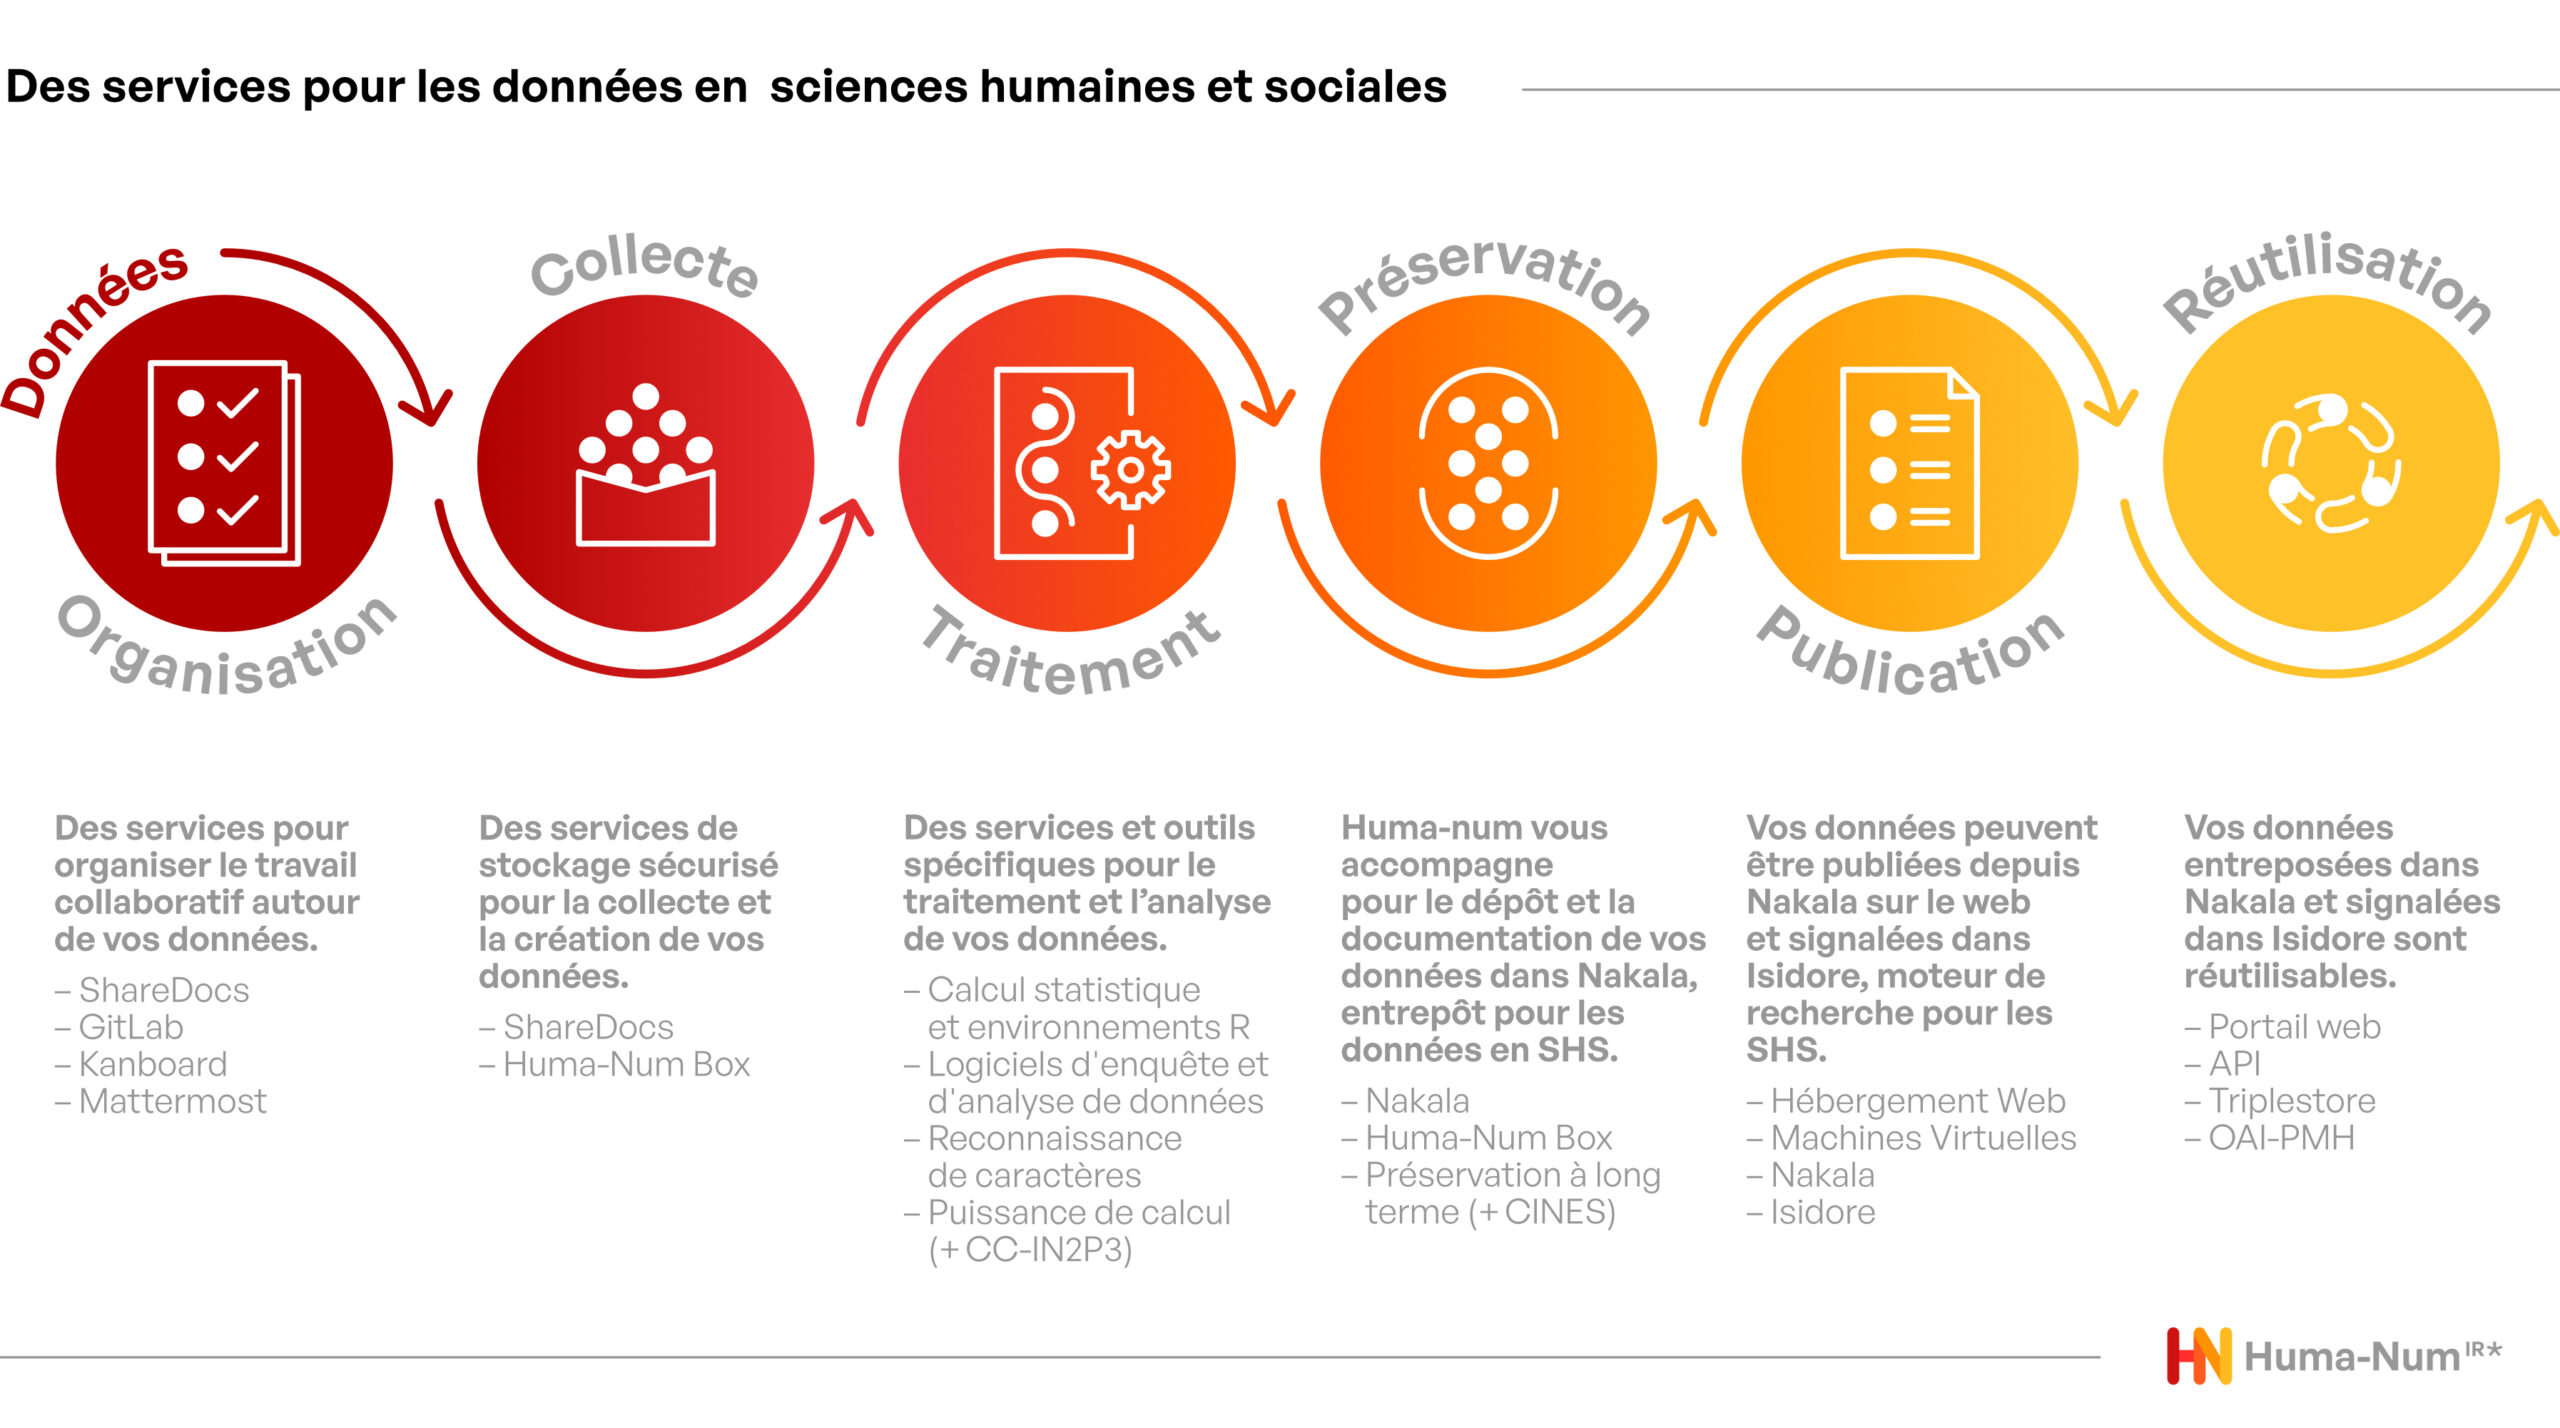
\includegraphics{IMG/Schema-du-cycle-de-vie-des-donnees-HN_2023_FR-2-scaled.jpg}

\subsection{\texorpdfstring{Des \textbf{consortiums} thématiques pour
collaborer, échanger, partager, élaborer des méthodologies, publier des
guides ou des thésaurus, organiser des formations ou des journées
d'études}{Des consortiums thématiques pour collaborer, échanger, partager, élaborer des méthodologies, publier des guides ou des thésaurus, organiser des formations ou des journées d'études}}\label{des-consortiums-thuxe9matiques-pour-collaborer-uxe9changer-partager-uxe9laborer-des-muxe9thodologies-publier-des-guides-ou-des-thuxe9saurus-organiser-des-formations-ou-des-journuxe9es-duxe9tudes}

\begin{figure}

\begin{minipage}{0.33\linewidth}

\includegraphics{IMG/Pictoria-200x70.jpg}\end{minipage}%
%
\begin{minipage}{0.33\linewidth}

\includegraphics{IMG/Logo_ARIANE-200x86.jpg}\end{minipage}%
%
\begin{minipage}{0.33\linewidth}

\includegraphics{IMG/logo-3DHN-200x52.png}\end{minipage}%
\newline
\begin{minipage}{0.33\linewidth}

\includegraphics{IMG/logo-PTM-png-200x80.png}\end{minipage}%
%
\begin{minipage}{0.33\linewidth}

\includegraphics{IMG/logo_MASAplus-200x81.png}\end{minipage}%
%
\begin{minipage}{0.33\linewidth}

\includegraphics{IMG/LOGO-DISTAM-sans-texte-200x158.png}\end{minipage}%
\newline
\begin{minipage}{0.33\linewidth}

\includegraphics{IMG/logo-canevas_png-200x127.png}\end{minipage}%
%
\begin{minipage}{0.33\linewidth}

\includegraphics{IMG/Musica-2-1-200x119.png}\end{minipage}%
%
\begin{minipage}{0.33\linewidth}

\includegraphics{IMG/logo-CORLI-png.png}\end{minipage}%
\newline
\begin{minipage}{0.33\linewidth}

\includegraphics{IMG/logo-sol-picto-194x200.png}\end{minipage}%

\end{figure}%

\begin{center}\rule{0.5\linewidth}{0.5pt}\end{center}

\emph{Site réalisé avec \href{https://quarto.org/}{Quarto}}.

\part{Histoire et Consortiums}

\phantomsection\label{consort}

\chapter{Historique}\label{historique}

\begin{itemize}
\tightlist
\item
  source officielle :
\end{itemize}

\begin{quote}
\section{L'historique}\label{lhistorique}

\begin{quote}
{[}\url{https://www.huma-num.fr/quest-ce-que-l-ir-huma-num/}{]}
\end{quote}

Huma-Num est le produit de la fusion au 1er mars 2013 de deux
infrastructures : le très grand équipement \textbf{Adonis} (TGE) et
l'infrastructure de recherche \textbf{Corpus} (IR).


\includegraphics{IMG/tge-adonis-2-300x52.png}

En mars 2007, \textbf{Adonis} (\emph{Accès unifié aux données et
documents numériques des sciences humaines et sociales}) est créé avec
l'objectif de réaliser un accès unifié aux données en SHS. Le projet du
TGE Adonis repose sur l'existence de données numériques structurées
selon des schémas identifiables et acceptés par les communautés
scientifiques productrices de données. L'\textbf{interopérabilité} des
données constitue de ce fait \textbf{une notion clef dans les
dispositifs d'infrastructures SHS}.
\end{quote}

\chapter{Les consortiums actifs}\label{les-consortiums-actifs}

\begin{figure}

\begin{minipage}{0.33\linewidth}

\includegraphics{IMG/Pictoria-200x70.jpg}\end{minipage}%
%
\begin{minipage}{0.33\linewidth}

\includegraphics{IMG/Logo_ARIANE-200x86.jpg}\end{minipage}%
%
\begin{minipage}{0.33\linewidth}

\includegraphics{IMG/logo-3DHN-200x52.png}\end{minipage}%
\newline
\begin{minipage}{0.33\linewidth}

\includegraphics{IMG/logo-PTM-png-200x80.png}\end{minipage}%
%
\begin{minipage}{0.33\linewidth}

\includegraphics{IMG/logo_MASAplus-200x81.png}\end{minipage}%
%
\begin{minipage}{0.33\linewidth}

\includegraphics{IMG/LOGO-DISTAM-sans-texte-200x158.png}\end{minipage}%
\newline
\begin{minipage}{0.33\linewidth}

\includegraphics{IMG/logo-canevas_png-200x127.png}\end{minipage}%
%
\begin{minipage}{0.33\linewidth}

\includegraphics{IMG/Musica-2-1-200x119.png}\end{minipage}%
%
\begin{minipage}{0.33\linewidth}

\includegraphics{IMG/logo-CORLI-png.png}\end{minipage}%
\newline
\begin{minipage}{0.33\linewidth}

\includegraphics{IMG/logo-sol-picto-194x200.png}\end{minipage}%

\end{figure}%

\chapter{Les consortiums cloturés}\label{les-consortiums-cloturuxe9s}

\part{Les services}

\phantomsection\label{service}

\chapter{Utiliser et produire des données
FAIR}\label{utiliser-et-produire-des-donnuxe9es-fair}

\cleardoublepage
\phantomsection
\addcontentsline{toc}{part}{Appendices}
\appendix

\chapter*{References
bibliographiques}\label{references-bibliographiques}
\addcontentsline{toc}{chapter}{References bibliographiques}

\markboth{References bibliographiques}{References bibliographiques}

\phantomsection\label{refs}
\begin{CSLReferences}{0}{1}
\bibitem[\citeproctext]{ref-QuestceQueLIR}
{«~Qu'est-ce que l'IR* Huma-Num\,? -- Huma-Num~»}. En ligne :
\url{https://www.huma-num.fr/quest-ce-que-l-ir-huma-num/} {[}consulté le
16 novembre 2024{]}.

\end{CSLReferences}




\end{document}
